\chapter{Implementation}
\label{Chapter4}


\section{Technologies Used}
The implementation of the split key wallet protocol and mobile authenticator for the Züs platform involves the following technologies:
\begin{itemize}
    \item Programming Languages: The core components of the system are implemented using Golang and Solidity programming languages.
    \item Cryptographic Libraries: The BLS signature scheme is implemented using the Apache Milagro Cryptographic Library (AMCL), which provides efficient implementations of pairing-based cryptography.
    \item Mobile Development Framework: The mobile authenticator is developed using the native Android, iOS and electron framework, enabling support for iOS, Android and Desktop devices.
    \item Secure Storage: The key components and sensitive data are stored securely using hardware-backed keystores, such as the Secure Enclave on iOS and the Keystore on Android.
\end{itemize}


\section{Smart Contract Development}
The Züs platform utilizes smart contracts to facilitate decentralized storage and cryptocurrency transactions. The split key wallet protocol is integrated into the existing smart contract infrastructure. The main modifications include:
\begin{itemize}
    \item Signature Verification: The smart contracts are updated to support the verification of BLS signatures, ensuring the integrity of transactions.
    \item Key Management: The smart contracts handle the registration and management of public keys associated with the split key wallets.
\end{itemize}


\section{Wallet Integration}
The split key wallet protocol is integrated into the existing Züs wallet implementation. The main changes include:
\begin{itemize}
    \item Key Generation: The wallet is modified to generate BLS key pairs and split the private key into multiple components.
    \item Partial Signature Generation: The wallet is updated to generate partial signatures using the key component stored on the primary device.
    \item Communication with Mobile Authenticator: The wallet establishes a secure communication channel with the mobile authenticator for transmitting partial signatures and receiving the final signature.
\end{itemize}


\section{Mobile Authenticator Development}
The mobile authenticator is developed as a standalone mobile application using the Native frameworks for each platform. The main components of the mobile authenticator include:
\begin{itemize}
    \item User Interface: The user interface is designed to provide a seamless and intuitive experience for authentication and transaction approval.
    \item Biometric Authentication: The mobile authenticator integrates biometric authentication (e.g., fingerprint or facial recognition) to ensure the security of user interactions.
    \item Secure Storage: The key component and other sensitive data are stored securely using the hardware-backed keystore available on the mobile device.
    \item Push Notifications: The mobile authenticator integrates with the Züs platform's notification system to receive real-time alerts for pending transaction approvals.
\end{itemize}

\subsection{Wallet Setup Process}
Figure \ref{fig:setup} illustrates the process of setting up a split key wallet in the Züs platform. The user initiates the setup by starting the desktop application, which generates a QR code containing the server IP address. The mobile wallet scans this QR code to establish a connection with the desktop application.

The original wallet key is used to create two keys - one stored on the mobile device and the other sent securely to the desktop application. After the key split is complete, the original key is deleted from the mobile wallet for enhanced security. A confirmation is sent back to the user indicating the successful setup of the split key wallet.

\begin{figure}[h]
    \centering
    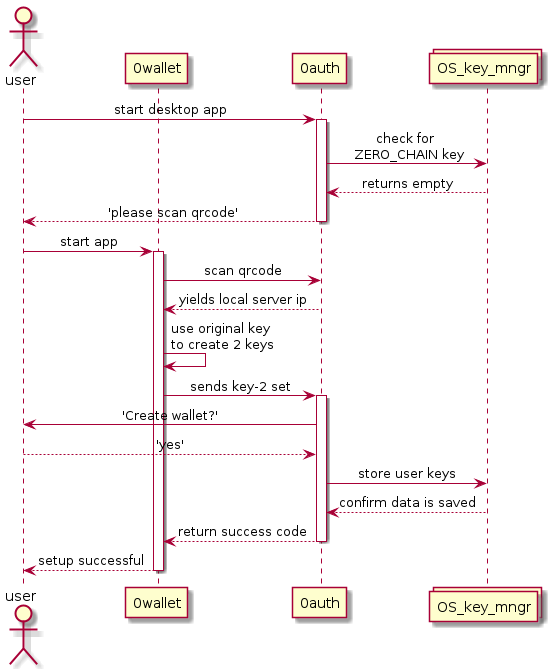
\includegraphics[width=\textwidth]{Images/setup_diagram.png}
    \caption{Split Key Wallet Setup Process}
    \label{fig:setup}
\end{figure}

Figure \ref{fig:setup_desktop} shows the user interface of the mobile wallet (left) and desktop authenticator (right) during the wallet setup process. The mobile wallet displays instructions for setting up the authenticator, including downloading the desktop application, scanning the QR code, and confirming the setup. The desktop authenticator presents the QR code for the mobile wallet to scan, establishing the connection between the two devices.

\begin{figure}[h]
    \centering
    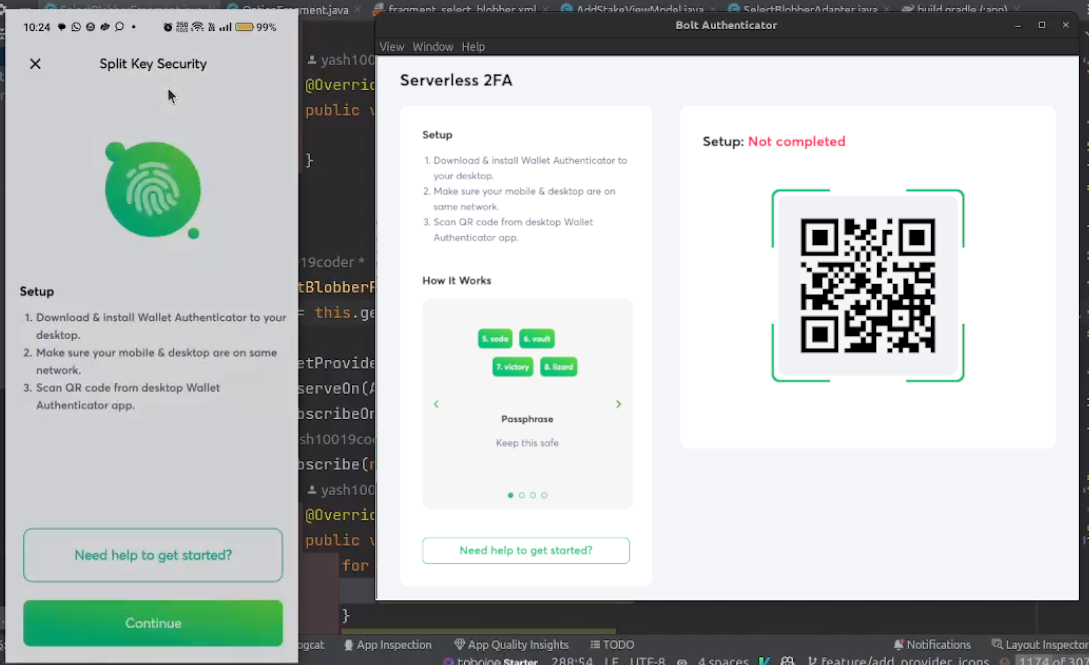
\includegraphics[width=\textwidth]{Images/setup_desktop.png}
    \caption{Mobile Wallet (left) and Desktop Authenticator (right) during Wallet Setup}
    \label{fig:setup_desktop}
\end{figure}

Figure \ref{fig:setup_mobile} shows the mobile wallet interface during the setup process. The user is prompted to scan the QR code displayed on the desktop authenticator to establish the connection. Once the connection is established, the key splitting process is initiated, and a success message is displayed upon completion.

\begin{figure}[h]
    \centering
    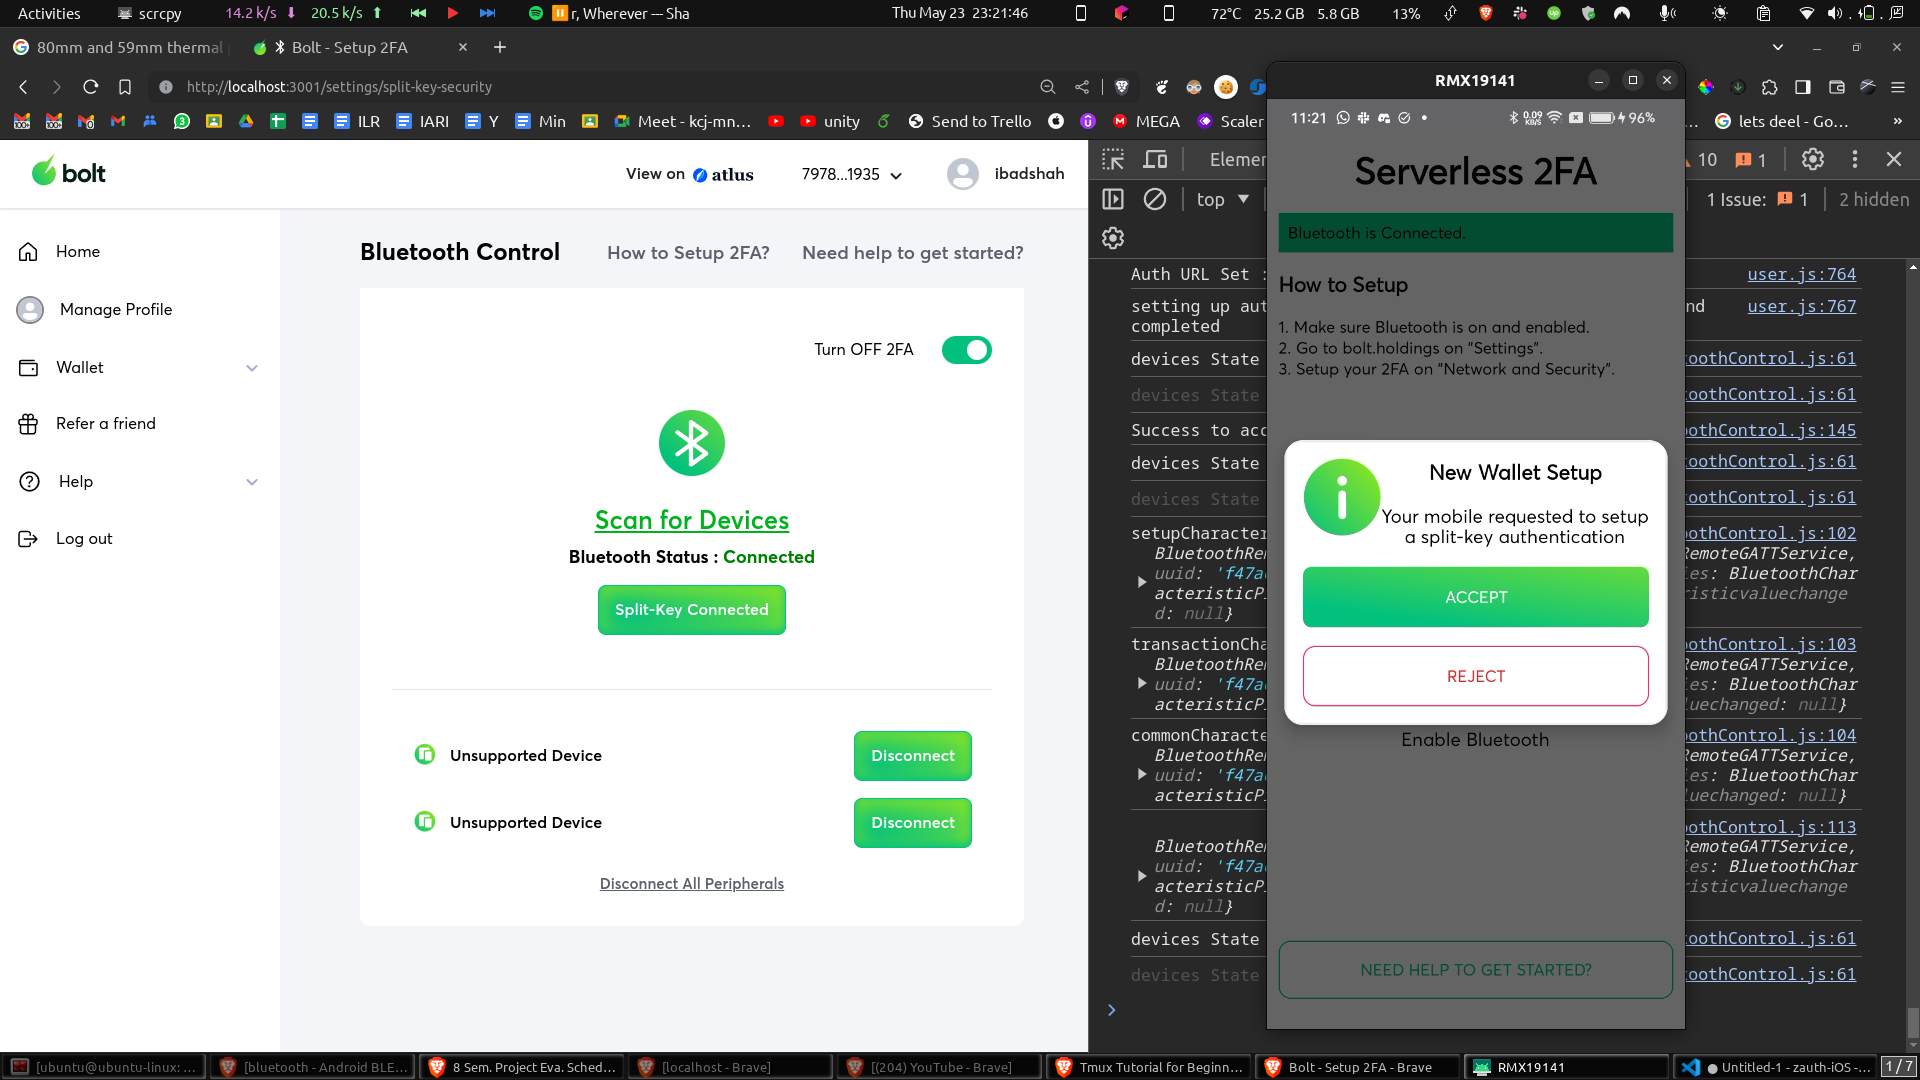
\includegraphics[width=\textwidth]{Images/setup_mobile.png}
    \caption{\href{https://bolt.holdings}{Bolt Web App (left)} Mobile Wallet Setup Process (right)}
    \label{fig:setup_mobile}
\end{figure}

Figure \ref{fig:setup_confirm} Once the mobile wallet scans the QR code, it sends a setup request to the desktop authenticator. The user is prompted to accept or reject the setup request on the desktop application (Figure \ref{fig:setup_confirm}). If accepted, the key splitting process is initiated, and a success message is displayed on the mobile wallet upon completion.

\begin{figure}[h]
    \centering
    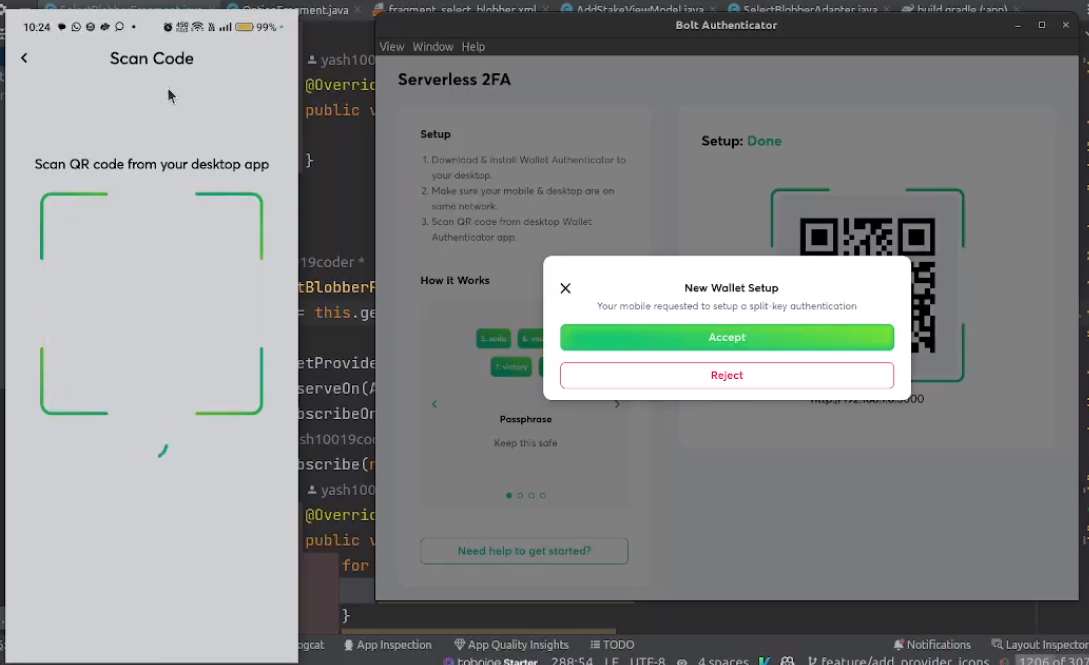
\includegraphics[width=\textwidth]{Images/setup_confirm}
    \caption{Split Key Setup Confirmation on Desktop Authenticator}
    \label{fig:setup_confirm}
\end{figure}

Figure \ref{fig:setup_success} shows the success message displayed on the mobile wallet after the key splitting process is completed successfully. The user is informed that the split key wallet has been set up and is ready for use. (Figure \ref{fig:setup_success}).

\begin{figure}[h]
    \centering
    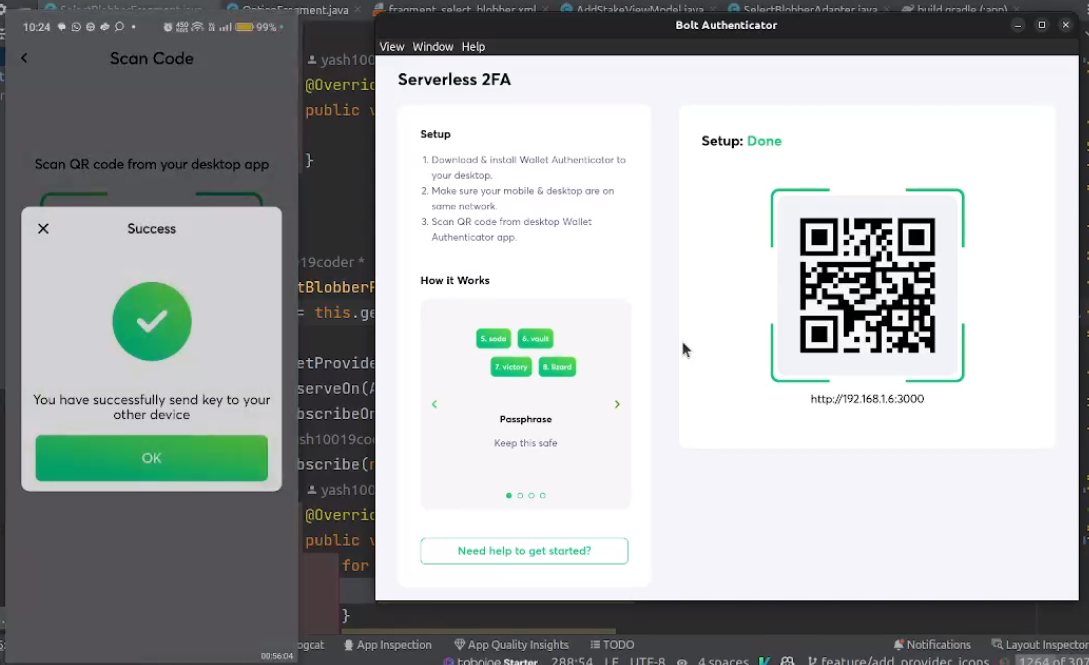
\includegraphics[width=\textwidth]{Images/setup_success}
    \caption{Split Key Wallet Setup Success Message}
    \label{fig:setup_success}
\end{figure}

\subsection{Transaction Signing Process}
Figure \ref{fig:transaction} depicts the transaction signing process using the split key wallet. When the user initiates a transaction from the mobile wallet, it is first signed with Key-1 stored on the mobile device. The partially signed transaction is then sent to the desktop application (0auth) for the second signature.

The user is prompted to confirm the transaction details on the desktop application. Upon confirmation, the transaction is signed with Key-2 stored securely in the desktop environment. The fully signed transaction, now containing signatures from both the mobile and desktop components, is returned to the mobile wallet. After verifying the signatures, the mobile wallet sends the transaction to the 0chain network for processing. This two-factor authentication process adds an extra layer of security to the user's transactions.

\begin{figure}[h]
    \centering
    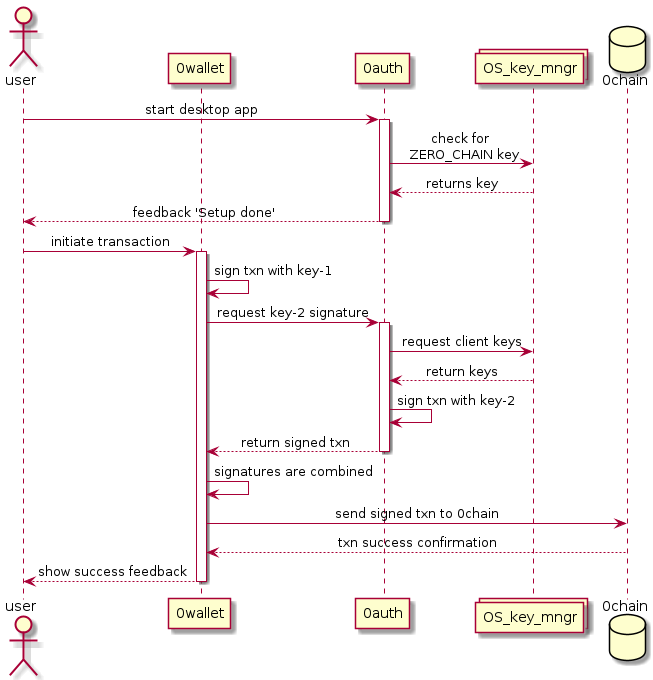
\includegraphics[width=\textwidth]{Images/transaction_diagram.png}
    \caption{Split Key Wallet Transaction Signing Process}
    \label{fig:transaction}
\end{figure}

Figure~\ref{fig:transaction_screen1} illustrates the initial step of the transaction signing process using the split key wallet. When the user initiates a transaction, such as staking tokens, from the mobile wallet, a signing request is sent to the desktop authenticator (0auth).

\begin{figure}[h]
    \centering
    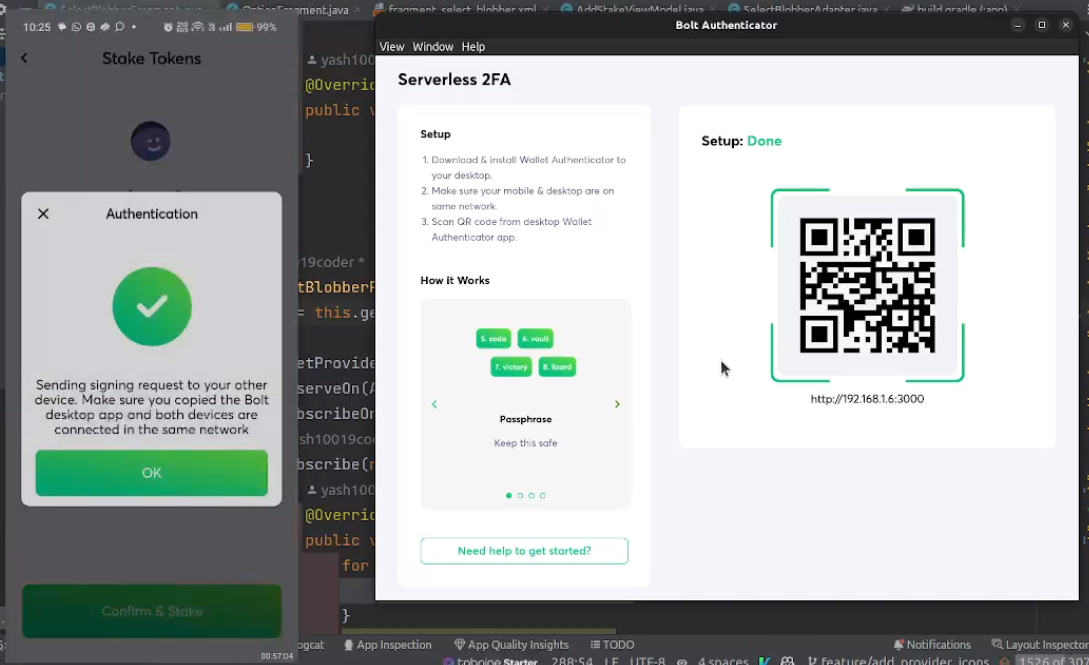
\includegraphics[width=\textwidth]{Images/transaction_initiation}
    \caption{Mobile Wallet: Sending signing request to desktop authenticator}
    \label{fig:transaction_screen1}
\end{figure}

In Figure \ref{fig:transaction_screen1}, the mobile wallet displays the option to "Confirm & Stake" tokens. Once the user initiates the staking process, a signing request is sent to the desktop authenticator, as indicated by the message "Sending signing request to your other device."

Figure \ref{fig:transaction_screen2} shows the desktop authenticator (0auth) displaying the transaction details for the user to review and approve or reject the transaction.

\begin{figure}[h]
    \centering
    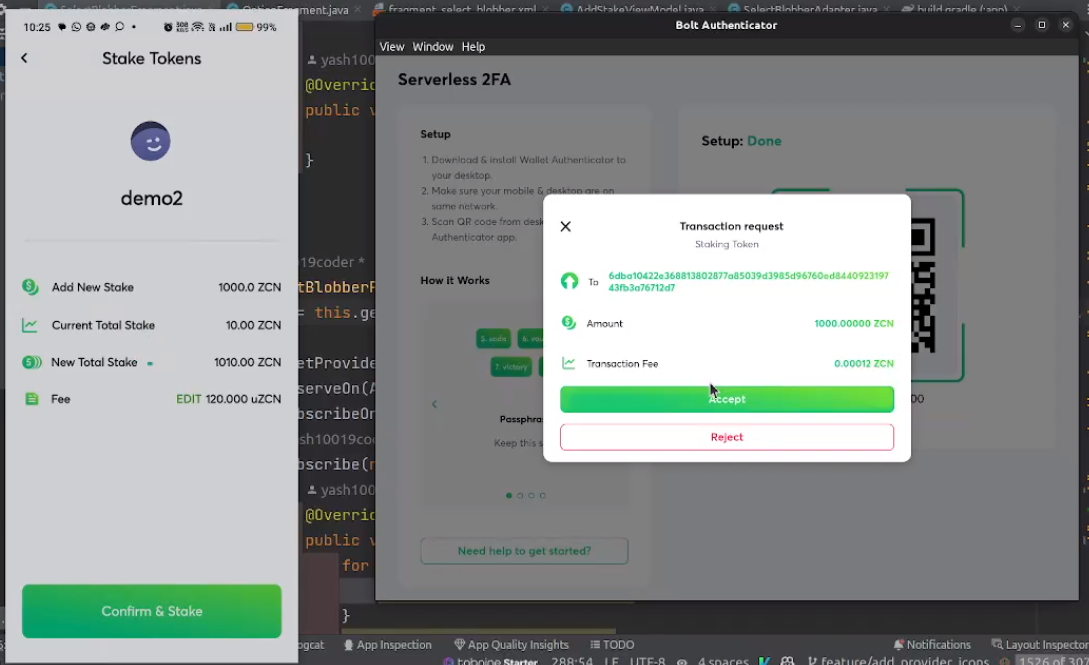
\includegraphics[width=\textwidth]{Images/transaction_confirmation}
    \caption{Desktop Authenticator: Transaction details for approval}
    \label{fig:transaction_screen2}
\end{figure}

On the desktop authenticator, the user is presented with the transaction details, including the recipient address, amount, and transaction fee. The user can review the transaction details and either accept or reject the transaction by clicking the respective button.

If the user accepts the transaction, the desktop authenticator signs the transaction using the key component stored securely on the desktop environment. The fully signed transaction, now containing signatures from both the mobile and desktop components, is sent back to the mobile wallet.

Finally, Figure \ref{fig:transaction_screen3} displays the confirmation message on the mobile wallet, indicating the successful completion of the staking process.

\begin{figure}[h]
    \centering
    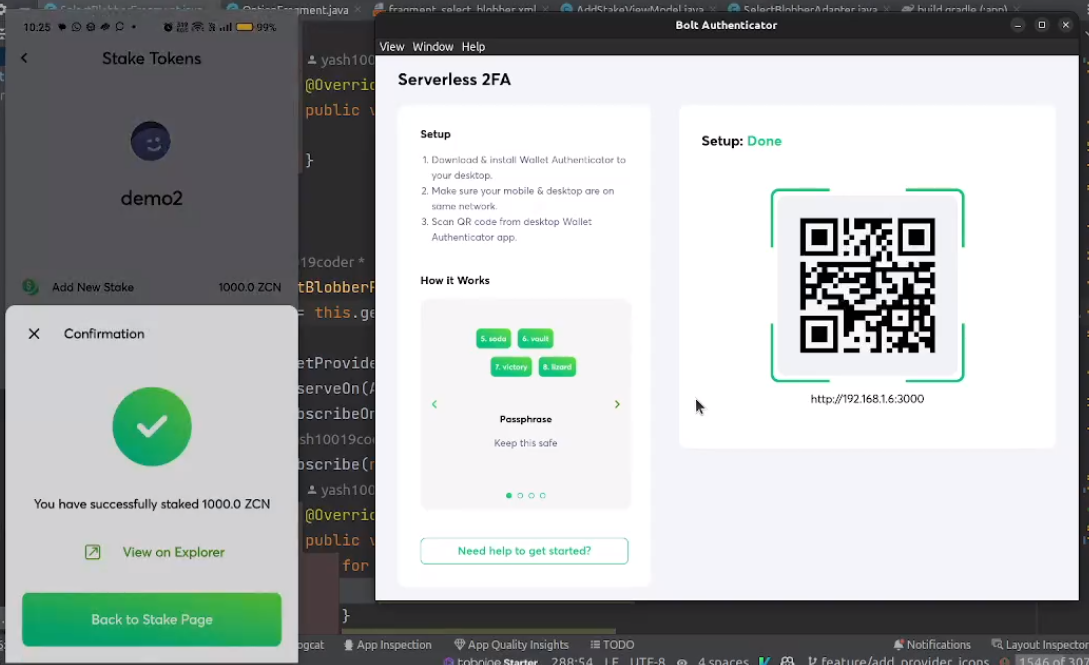
\includegraphics[width=\textwidth]{Images/transaction_success}
    \caption{Mobile Wallet: Confirmation of successful staking}
    \label{fig:transaction_screen3}
\end{figure}

In Figure \ref{fig:transaction_screen3}, the mobile wallet displays a confirmation message indicating the successful staking of the specified token amount. The user can choose to view the transaction details on the explorer or return to the stake page.

This two-factor authentication process, involving both the mobile wallet and the desktop authenticator, adds an extra layer of security to the user's transactions by requiring approval from both devices.


\section{Integration Testing}
Rigorous integration testing is performed to ensure the smooth functioning of the split key wallet protocol and mobile authenticator within the Züs platform. The testing scenarios include:
\begin{itemize}
    \item Key Generation and Splitting: Verifying the correctness of key generation and the splitting of the private key into multiple components.
    \item Transaction Signing: Testing the end-to-end process of initiating a transaction, generating partial signatures, and combining them to produce the final signature.
    \item Mobile Authenticator Functionality: Validating the mobile authenticator's user interface, biometric authentication, secure storage, and push notification capabilities.
    \item Error Handling and Recovery: Testing various error scenarios, such as network disruptions or device failures, and ensuring proper error handling and recovery mechanisms are in place.
\end{itemize}

The implementation phase involves close collaboration between the development team and the Züs platform stakeholders to ensure seamless integration and adherence to the platform's security and performance requirements.
